%%%% Preamble
\documentclass[paper=a4,fontsize=11pt]{report}


%\begin{document}

%\begin{titlepage}
    
\newcommand{\HRule}{\rule{\linewidth}{0.5mm}} % Defines a new command for the horizontal lines, change thickness here
    
\center % Center everything on the page
     
%----------------------------------------------------------------------------------------
%	HEADING SECTIONS
%----------------------------------------------------------------------------------------
    
\textsc{\LARGE Instituto Tecnológico de Buenos Aires}\\[2cm] % Name of your university/college
\textsc{\Large Electronica III}\\[1.5cm] % Major heading such as course name
\textsc{\large Trabajo Práctico N° 2}\\[0.5cm] % Minor heading such as course title
    
%----------------------------------------------------------------------------------------
%	TITLE SECTION
%----------------------------------------------------------------------------------------
    
\HRule \\[0.5cm]
{ \huge \bfseries Trabajo Práctico de Laboratorio Nr. 2}\\[0.4cm] % Title of your document
\HRule \\[2cm]
     
%----------------------------------------------------------------------------------------
%	AUTHOR SECTION
%----------------------------------------------------------------------------------------
    
\begin{minipage}{0.4\textwidth}
\begin{flushleft} \large
\emph{Grupo 2:}\\		%names
[.3cm]
Victor \textsc{Oh}\\
Leg. ???\\ 
[.3cm]
Ian \textsc{Diaz}\\
Leg. ???\\ 
[.3cm]
Benjamín Carlos \textsc{Lin}\\
Leg. 57242 \\ 
[.3cm]
Malena \textsc{Muller}\\
Leg. ???\\ 
[.3cm]
\end{flushleft}
\end{minipage}
~
\begin{minipage}{0.4\textwidth}
\begin{flushright} \large
%\emph{Profesor:} \\
%[.3cm]
%Pablo  \textsc{Cossutta}\\ % Supervisor's Name
%Alejandra \textsc{Weill} \\% Supervisor's Name
%Matías  \textsc{Salvati} % Supervisor's Name
\end{flushright}
\end{minipage}\\[2cm]
    
%----------------------------------------------------------------------------------------
%	DATE SECTION
%----------------------------------------------------------------------------------------
    
\vfill
{\large Entregado: 17 de Octubre de 2018}\\[2cm]
    
\vfill 
    
\end{titlepage}
%
%\pagenumbering{roman}
%\tableofcontents
%\newpage
%\pagenumbering{arabic}
%
%Test Text

\section{\color{olive}Exercise 5: Compatibility between TTL and CMOS}

\subsection{\color{purple}Floating input in TTL and CMOS}

Connecting the following circuit in figure \ref{fig:ej5ttl} and \ref{fig:ej5cmos} leaving one of the inputs floating having $Vcc = 5V$. 

\begin{figure}[h!]
         \begin{minipage}{.47\linewidth}
        \centering
        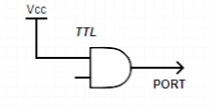
\includegraphics[width=.6\linewidth]{../Exercise5/TTL5.png}
        \caption{\color{cyan}Floating TTL}
        \label{fig:ej5ttl}
        \end{minipage}
         \begin{minipage}{.5\linewidth}
        \centering
        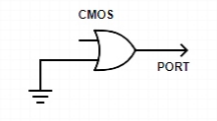
\includegraphics[width=.5\linewidth]{../Exercise5/CMOS5.png}
        \caption{\color{cyan}Floating CMOS}
        \label{fig:ej5cmos}
    \end{minipage}
\end{figure}

For the 74LS08, the TTL component, the output port value shown was a logical 1 constantly. On the other hand, the 74HC32, the CMOS component, the results were random with a frequency of 50Hz, having a quadratic function from 0 to 5V or 3 to 5V or a 0 to 0.8V amplitude function.

\begin{figure}[h!]
        \centering
        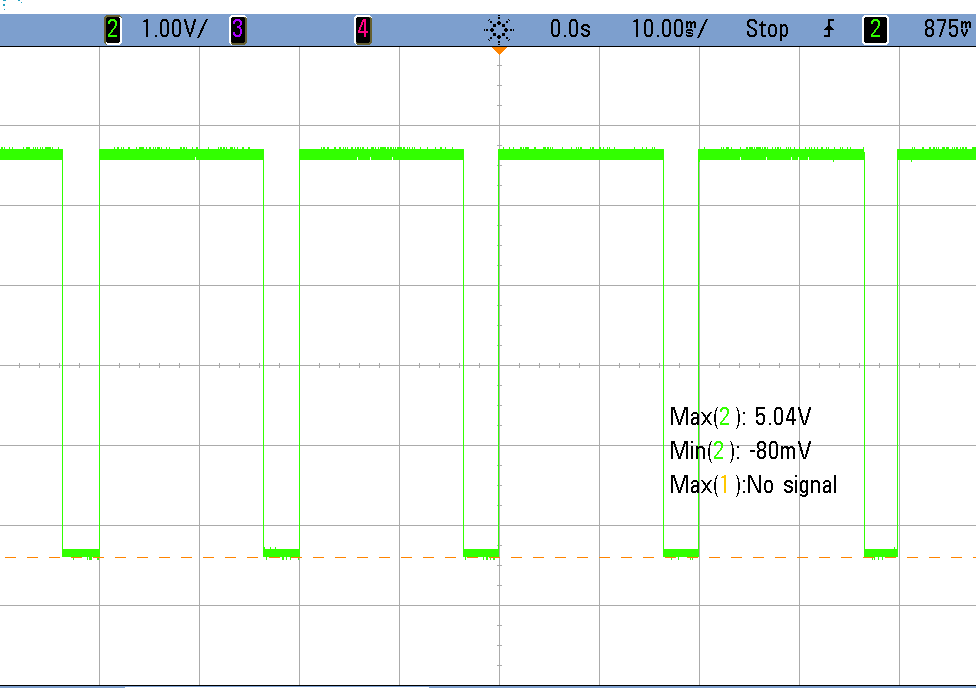
\includegraphics[scale=0.19]{../Exercise5/cmos_cerda2.png}\hspace{1cm}
%        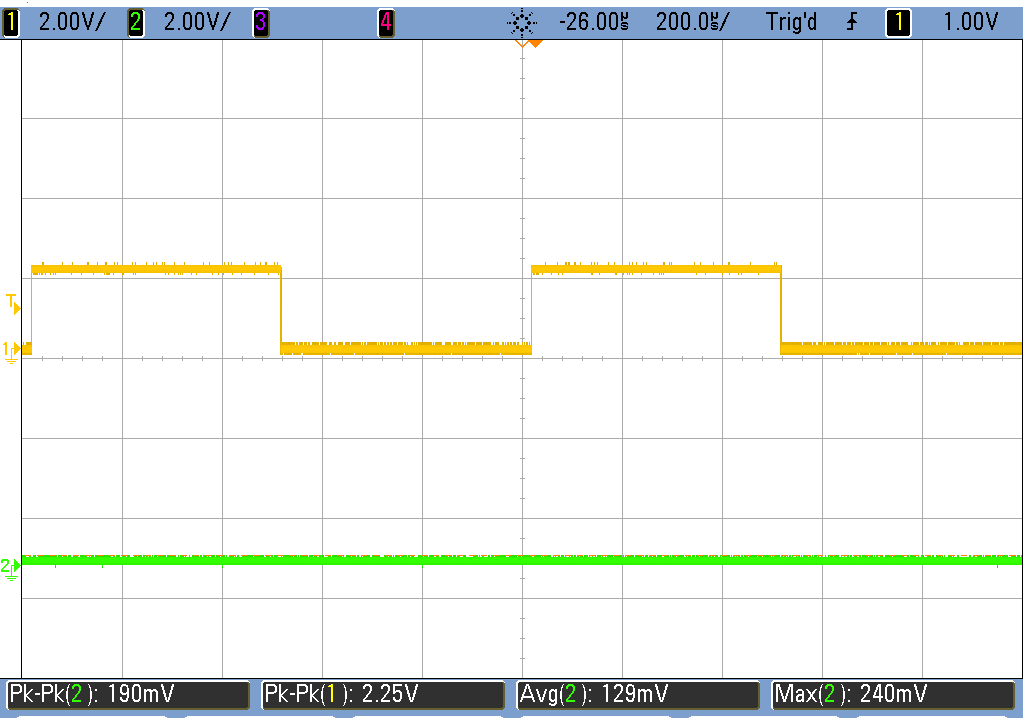
\includegraphics[scale=0.19]{HC-LS-2V.png}\\
        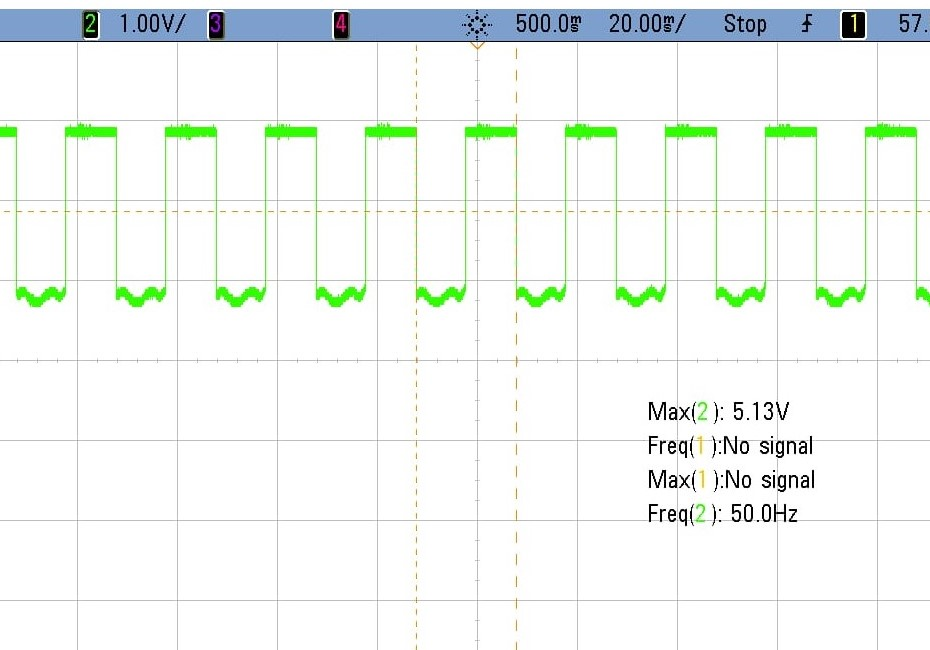
\includegraphics[scale=0.2]{../Exercise5/cmos_dads.jpeg}\\
		\vspace{0.2cm}
%		\hspace{0.9cm}
	   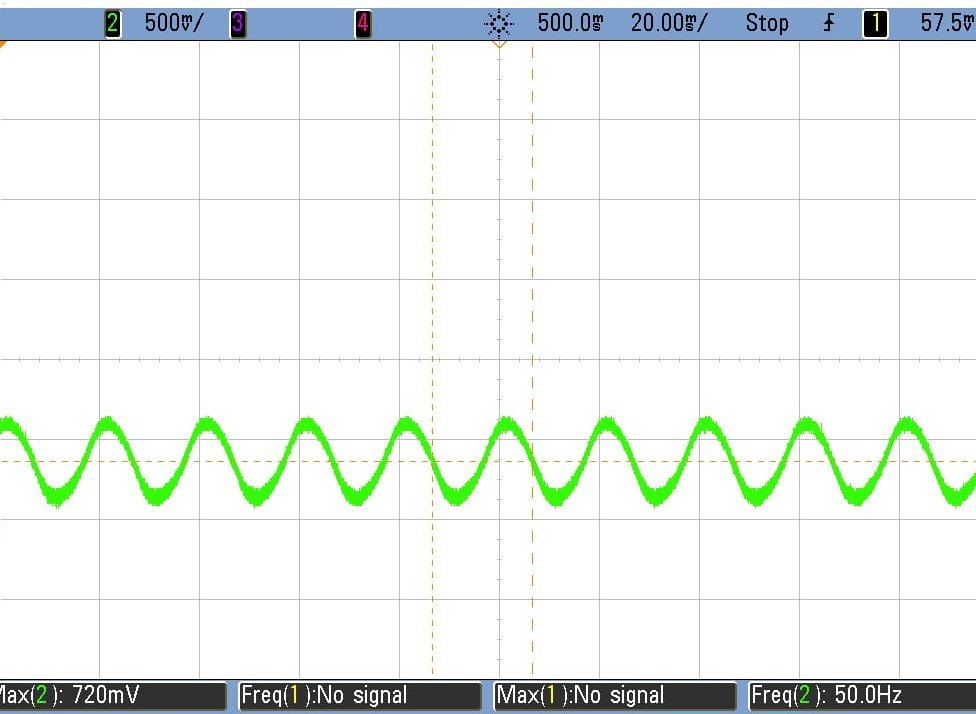
\includegraphics[scale=0.19]{../Exercise5/cmos_ahifdas.jpeg} 
%        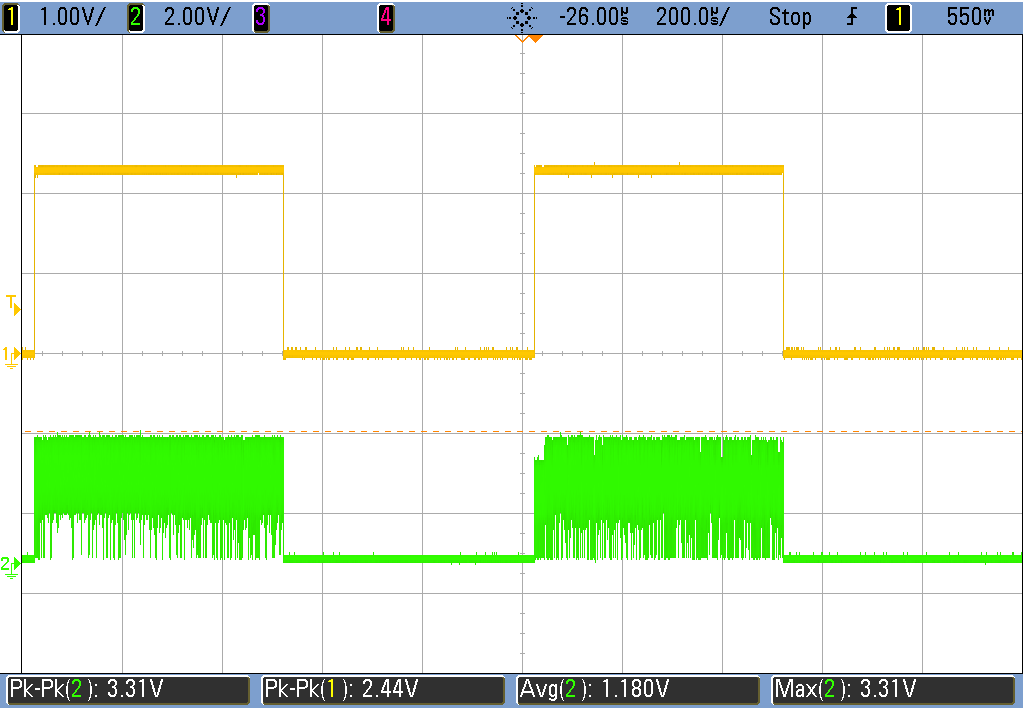
\includegraphics[scale=0.19]{HC-LS-2p3V.png}
        \caption{\color{cyan}74HC02 load to 74LS02}
        \label{fig:ej2exhctols}
    \end{figure}

The reason for this variation in CMOS could be explain by the high impedance at the input making the floating pin induce electric current by noise, creating random values to the output. For this reason, it is recommended in the data-sheet to connect the floating input to the GND or to Vcc depending to the situation, so that unexpected variations wouldn't affect the measurements.

\subsection{\color{purple}TTL loaded to CMOS}

Having the TTL loaded to CMOS as the following figure, with a input value being a quadratic function. 

\begin{figure}[h!]
        \centering
        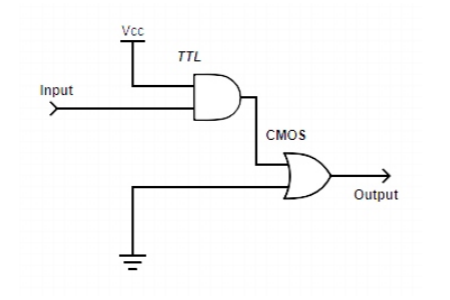
\includegraphics[scale=0.6]{../Exercise5/cir5.png}
        \caption{\color{cyan}TTL loaded to CMOS circuit}
        \label{fig:ej5cir}
\end{figure}

\pagebreak

When the TTL output value is a logical 1, a voltage from 2.4 to 5V is generated. But there is a problem within this values because the input values for a 1 in CMOS components is from 3.15 to 5V, so in the range of 2.4 to 3.15V the input value for the CMOS is undefined which may causing problems while measuring the two components loaded.

\begin{figure}[h!]
        \centering
        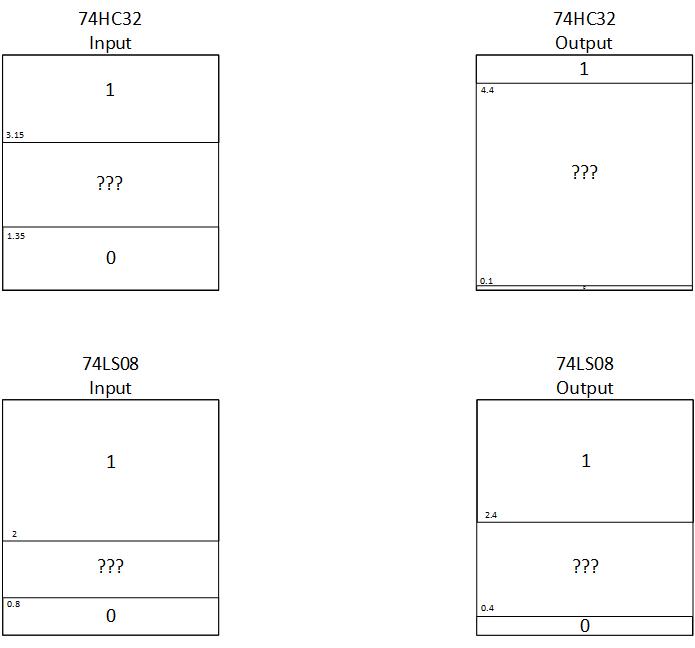
\includegraphics[scale=0.45]{../Exercise5/Graficos5.png}
        \caption{\color{cyan}Theoretical input and output noise margins}
        \label{fig:ej5noisemargin}
\end{figure}

A solution to this problem may be utilizing the same technology components, this is to say using only TTL or CMOS, so that the defined values of the output from the first component is always in range of the input values in the second one. Another solution for this could be utilizing a HCT integrated circuit, a CMOS sub-family, which can make possible the the compatibility between TTL and CMOS by having the following noise margin characteristics. 

\begin{figure}[h!]
        \centering
        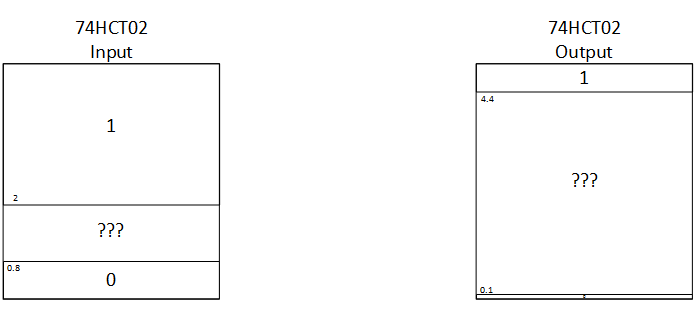
\includegraphics[scale=0.45]{../Exercise5/dataaa5.png}
        \caption{\color{cyan}HCT noise margins}
        \label{fig:ej5noisemargin}
\end{figure}


%\end{document}